\begin{figure*}[p]
	\centering
	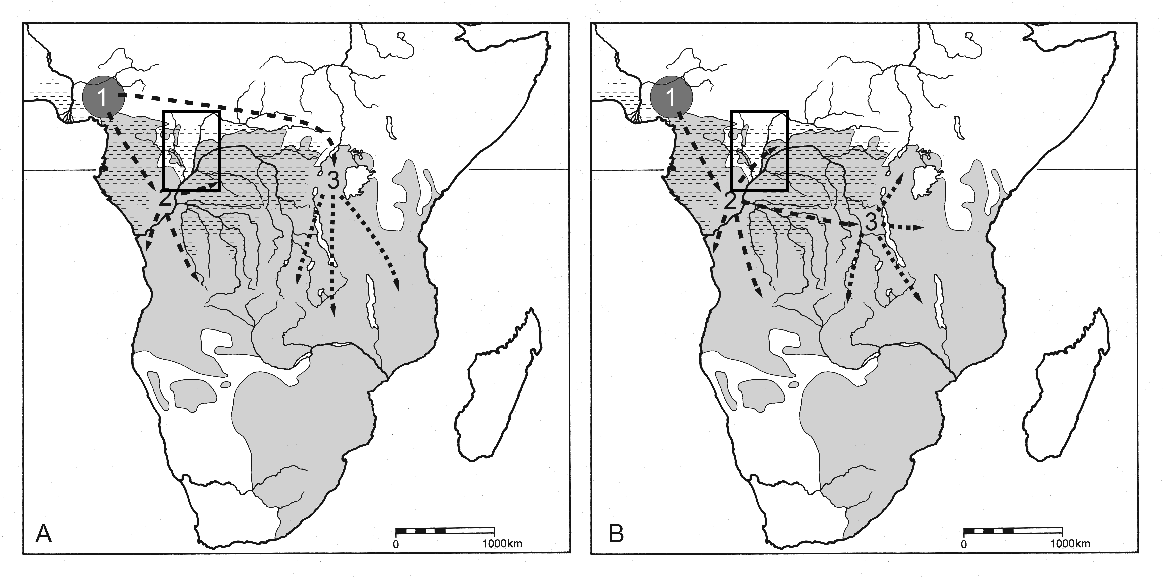
\includegraphics[width=\textwidth]{bib/Eggert2012/207Abb6.pdf}
	\caption{Bantuausbreitung: Gegenwärtig diskutierte Modelle zur Bantuausbreitung und das Arbeitsgebiet \parencites[rot; nach][57, Abb.~2]{Pakendorf.2011}[207 Abb.~6a/b]{Eggert.2012}.}
	\label{fig:Bantuexp_Eggert2012-207Abb6ab}
\end{figure*}


\begin{figure*}[p]
	\centering
	\includegraphics[width=.69\textwidth]{bib/deMaret2013/630Fig43-2.pdf}
	\caption{Bantuausbreitung: Ausbreitungsrouten \parencite[630 Abb. 43.2]{deMaret.2013} und das Arbeitsgebiet (rot).}
	\label{fig:Bantuexp_deMaret2013-630Fig43-2}
\end{figure*}

\section{Archäologie und Historische Linguistik}

Ein zentraler Forschungsgegenstand der Kulturgeschichte Afrikas südlich der Sahara ist die Ausbreitung der Bantu sprechenden Gruppen über fast den gesamten Raum südlich des Äquators: die \enquote*{Bantu-Expansion}. Bantu ist eine Sprachfamilie, der zwischen 300 und 680 einzelne Sprachen zugeordnet werden \parencites{Nurse.2003}[81]{Eggert.2016c}. Die hypothetische Urheimat dieser Sprachfamilie wird derzeit im Grenzgebiet von Kamerun und Nigeria -- im nordwestlichen Eck ihrer heutigen Verbreitung -- verortet (Abb.~\ref{fig:Bantuexp_Eggert2012-207Abb6ab}--\ref{fig:Bantuexp_deMaret2013-630Fig43-2})

Die Frage nach der Ausbreitung der Bantu-Sprachen im südlichen Afrika wurde über Jahrzehnten im Spannungsfeld von Linguistik und Archäologie diskutiert. Die Debatte wies jedoch bereits früh eine starke Vermischung linguistischer und archäologischer Argumente auf, was deutliche Zirkelschlüsse zur Folge hatte \parencites{Eggert.2005}[82]{Eggert.2016c}. Die seit einigen Jahren hinzukommenden Daten aus populationsgenetischen Untersuchungen führten nicht zu einem Aufbrechen dieses Dilemmas. Vielmehr führt die Populationsgenetik zu einer höheren Komplexität und spezifischen Interpretationslücken. So lassen sich auf genetischer Seite nur vertikale Vererbungen von Eltern zu Kindern nachvollziehen, während Sprachgemeinschaften, deren Untersuchung angestrebt ist, auch horizontale Beeinflussungen zulassen \parencite[86]{Eggert.2016c}. Aus diesem Umstand ergibt sich für \textcite{Eggert.2016c} eine Aufweitung des ursprünglichen Dilemmas zu einem Trilemma.

Zur Erklärung der Ausbreitung der Bantu-Sprachen postulieren nicht wenige Forscher mehr oder minder großräumige Wanderungsbewegungen \parencites{Vansina.1995}{Ehret.2001}. Für das Arbeitsgebiet werden eine Reihe linguistisch inspirierter historischer Hypothesen diskutiert \parencite[10f.; siehe Abb.~\ref{fig:Bantuexp_Eggert2012-207Abb6ab}--\ref{fig:Bantuexp_deMaret2013-630Fig43-2}]{Eggert.1992}. So geht \textcite{Ehret.1982} von einer sehr frühen Besiedlung des Regenwaldes durch Bantu-Sprecher aus. Basierend auf Überlegungen von \textcite{Heine.1973} datiert er die frühesten Phasen der Bantu-Expansion in den zentralen Teil des Regenwaldes -- auch in das gesamte Areal westlich des mittleren und unteren Ubangi-Flusses -- bereits an den Beginn des zweiten vorchristlichen Jahrtausends \parencite[58, 63~Karte 10; Abb.~\ref{fig:Bantuexp_deMaret2013-630Fig43-2}]{Ehret.1982}. Für \textcite[51f. Karten~2.7--2.8]{Vansina.1990} hingegen stellten die weiten Sumpfgebiete westlich des Ubangi eine deutliche Barriere für die Ausbreitung der Bantu-Sprecher dar. Er postuliert eine nördliche Ausweichbewegung der allgemein nach Osten gerichteten Ausbreitung des Bantu entlang der nördlichen Grenze des Regenwaldes und lässt die Sangha-Region undatiert (ebd. 51 Karte~2.7; Abb.~\ref{fig:Bantuexp_Eggert2012-207Abb6ab}).

Die Regenwaldgebiete Zentralafrikas sind vor allem deshalb von zentraler Bedeutung für die Annäherung an das Problem der Ausbreitung der Bantusprachen, ja geradezu \enquote{der entscheidende Prüfstein für die Rolle der Archäologie bei der Bantuausbreitung} \parencite[207]{Eggert.2012}, da sie aktuell fast vollständig von Bantu sprechenden Gruppen besiedelt sind und die Aufsiedlung durch keramikherstellende Gruppen im Inneren Kongobecken bereits plausibel mit der Bantu-Ausbreitung verknüpft wurde \parencite[244--246]{Wotzka.1995}. Beim gegenwärtigen Stand der archäologischen Erforschung Zentralafrikas müssen jedoch grundsätzlich alle Versuche, die historische Verbreitung beziehungsweise Ausbreitung kulturell-linguistischer Gruppen zu erfassen, als pure Spekulation bezeichnet werden \parencites[78]{David.1982}[105]{Boyd.2007}. Weder die Historische Linguistik noch die Populationsgenetik sind in der Lage generische Aussagen zur zeitlichen Dimension der jeweils beobachteten Phänomene zu machen \parencite[84]{Eggert.2016c}, dies vermag lediglich die Archäologie.\footnote{Umfassende kritische Auseinandersetzungen zum Spannungsfeld von Historischer Linguistik und Archäologie in der Frage der Bantu-Expansion finden sich bei \textcites{Eggert.2005}{Eggert.2012c}{Eggert.2012}{Eggert.2016c}.}

%\parencite{Bostoen.2015} Sangha-Korridor
%Die Sprachgeschichte des Arbeitsgebietes ... \todo{MEHR}
%>> Grodemund, Rebekka - kritisch würdigen (mündl. HPW 2015)
